\subsection{Class Diagram}
\noindent\makebox[\textwidth]{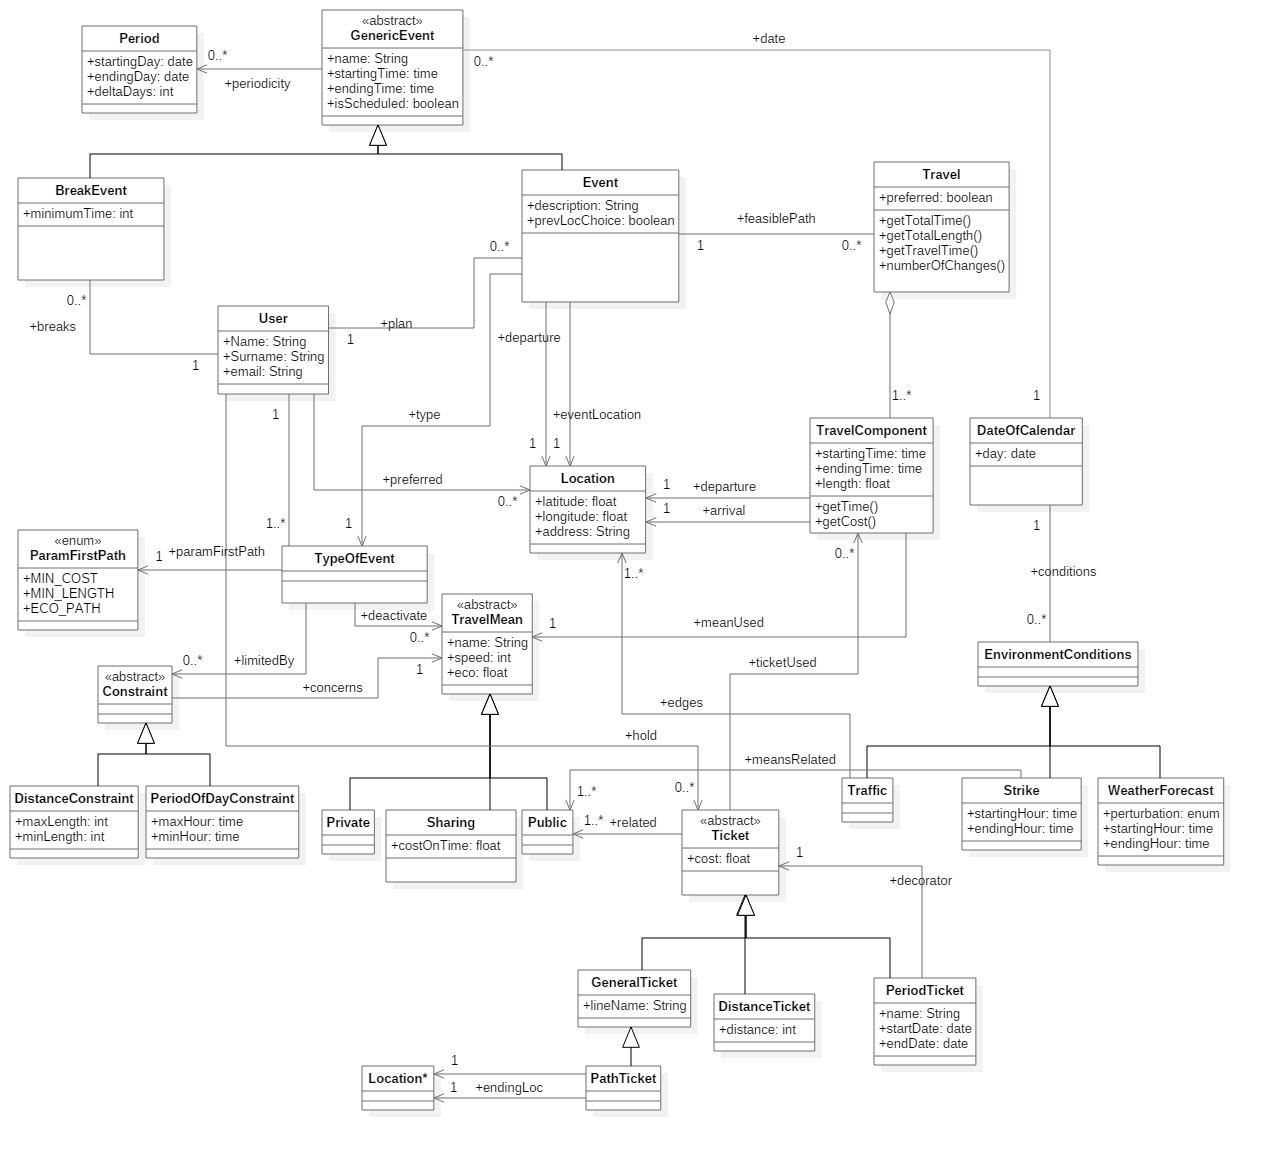
\includegraphics[width=\paperwidth,height=\paperheight,keepaspectratio]{class_diagram.jpg}}
\newline
An \textit{Event} is associated to one or more \textit{Travels}, a \textit{Travel} proposed requires the use of one or more \textit{Travel means}. The path of a \textit{Travel} that include different \textit{Travel Means} needs a structure where every \textit{Single Travel} (the path that can be performed with the same \textit{Travel Mean}), is memorized. Through a vector, an object of the \textit{Travel} class contains each \textit{Single Travel}.
\newline
\newline
\textit{Travel} class has the attribute \textit{preferred}: a Boolean value that identifies the path showed in the daily schedule for an inserted \textit{Event}. It must be checked that, for each \textit{Event}, only one \textit{Travel} is marked as preferred.
\newline
If a proposed path has different \textit{Single Travels}, information about time and length are provided by methods of the \textit{Travel} class that combine the values found in each related object of the\textit{Single Travel} class.
\newline
\newline
To represent \textit{Tickets} we use a hierarchy of classes: \textit{Distance Ticket} is used for tickets whose validity is indicated with a length, \textit{General Ticket} is used for particular tickets that allow the user to travel without constraints in a specified area, \textit{Path Ticket} is used when departure and arrival locations are indicated on the ticket. 
\newline
A \textit{Ticket} can be valid into specified dates or after the validation, for this reason the management of the time of validity is done with \textit{pattern Decorator}: it is used to specify the validity of an existing ticket.
